\newcounter{nuserstory}
\newcounter{nusecase}

\newcommand{\userstory}[4]{%
    \refstepcounter{nuserstory}
    \subsection{#1}
    \label{userstory:\thenuserstory}
    \hangindent=40pt
    \textbf{\textit{As a}} #2,\\
    \textbf{\textit{I want to}} #3,\\
    \textbf{\textit{so that}} #4.
}
\newenvironment{usecase}[1]
{
    \refstepcounter{nusecase}%
    \subsection{Use Case \thenusecase: #1}%
    \label{usecase:\thenusecase}%
}{}

\chapter{Requirement Analysis}
\label{chap:requirement-analysis}

\section{Stakeholder Analysis}
\label{section:stakeholder-analysis}

\begin{enumerate}[leftmargin=80pt]
    \item \textbf{Animators \& Video Artists:} The primary stakeholders are content creators and 
    video artists who want to protect their work from unauthorized AI training.
    \item \textbf{Regulatory \& Legal Bodies:} Government and industry groups ensuring 
    compliance with copyright laws, AI ethics, and intellectual property protection.
    \item \textbf{Cybersecurity \& Digital Rights Organizations:} Groups that focus on copyright protection, 
    AI misuse prevention, and ethical AI practices. They may promote or validate the effectiveness of Protractor.

\end{enumerate}

\section{User Stories}
\label{section:user-stories}

\userstory{Upload \& Protecting Video Content from AI Training%
}{digital content creator or video artist%
}{apply adversarial techniques to my videos to prevent AI models from copying my style%
}{I can protect my work from unauthorized AI training while keeping the video unchanged for humans}

\userstory{Ensuring Video Quality for Human Viewers%
}{digital content creator or video artist%
}{apply AI poisoning techniques without affecting the video’s visual quality for humans%
}{my audience can still enjoy my videos without noticeable distortions}

\userstory{Customizing Poisoning Parameters%
}{digital content creator or video artist%
}{adjust the poisoning settings such as intensity level and render quality before starting the process%
}{I can control how strongly the video is protected while balancing quality and performance}

\userstory{Processing Videos Efficiently%
}{content creator with large video files%
}{have my videos processed quickly without long waiting times%
}{I can protect my videos without delays affecting my workflow}

\userstory{Monitoring Poisoning Progress%
}{user waiting for video processing to complete%
}{see real-time updates on the status of my video poisoning%
}{I know how long the process will take and when my video will be ready}


\section{Use Case Diagram}
\label{section:use-case-diagram}

\begin{itemize}
    \item \textbf{\textit{User}}---A default group of users which has all the basic functionalities
\end{itemize}


\begin{itemize}
    \item \textbf{\textit{User}}---A default group of users which has all the basic functionalities
\end{itemize}


\section{Use Case Model}
\label{section:use-case-model}

\begin{usecase}{Uploading a Video}
    \textbf{Actors:} Pong (Digital Content Creator), Protractor (System)

    \textbf{Description:} Pong wants to upload a video file to the system in preparation for poisoning.

    \textbf{Scenario:}
    \begin{enumerate}[leftmargin=80pt]
        \item Pong opens the Protractor web application.
        \item System displays the upload interface.
        \item Pong selects a supported video format file and clicks the upload button.
        \item System validates the file and stores it for processing.
    \end{enumerate}
    \textbf{Alternative Flow:} If the file type is unsupported, the system displays an error message.
\end{usecase}

\begin{usecase}{Setting Poisoning Parameters}
    \textbf{Actors:} Pong (Digital Content Creator), Protractor (System)

    \textbf{Description:} Pong customizes the poisoning settings before starting the video poisoning process.

    \textbf{Scenario:}
    \begin{enumerate}[leftmargin=80pt]
        \item Pong navigates to the settings panel after uploading a video.
        \item System displays available poisoning parameters.
        \item Pong selects the settings.
        \item System saves the selected configuration for use in the next step.
    \end{enumerate}
\end{usecase}

\begin{usecase}{Starting the Poisoning Process}
    \textbf{Actors:} Pong (Digital Content Creator), Protractor (System)

    \textbf{Description:} After configuring the parameters, Pong starts the video poisoning process.

    \textbf{Scenario:}
    \begin{enumerate}[leftmargin=80pt]
        \item Pong clicks the "Start Poisoning" button.
        \item System begins poisoning the video.
        \item System displays a progress indicator or loading bar.
    \end{enumerate}
\end{usecase}

\begin{usecase}{Viewing the Poisoning Progress}
    \textbf{Actors:} Pong (Digital Content Creator), Protractor (System)

    \textbf{Description:} Pong wants to track the progress of the poisoning process.

    \textbf{Scenario:}
    \begin{enumerate}[leftmargin=80pt]
        \item System updates a progress are processed.
        \item Pong monitors the process status.
        \item Once complete, the system notifies Pong that the video is ready.
    \end{enumerate}
\end{usecase}

\begin{usecase}{Downloading the Poisoned Video}
    \textbf{Actors:} Pong (Digital Content Creator), Protractor (System)

    \textbf{Description:} Pong downloads the final poisoned video file to their device.

    \textbf{Scenario:}
    \begin{enumerate}[leftmargin=80pt]
        \item The system displays a "Download" button once poisoning is complete.
        \item Pong clicks the button to download the poisoned video.
        \item System sends the processed file to Pong’s device.
    \end{enumerate}
\end{usecase}


\section{User Interface Design}
\label{section:user-interface-design}
<TIP: Put the initial design of your application here. You can
showcase a detailed design of a specific page or a sitemap of your application.
See an example below./>

\begin{figure}[h]
    \centering
    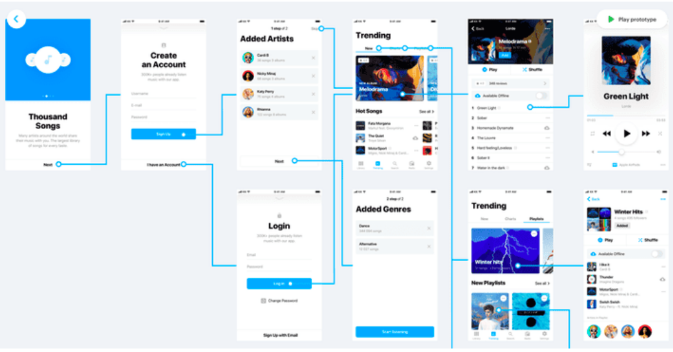
\includegraphics[width=0.8\textwidth]{examples/user-interface-design.png}
    \caption{User Interface Design}
\end{figure}